\section{Cálculo de Radioenlace Satelital} \label{sec:radioenlace}
El análisis y diseño del sistema de comunicaciones para la misión CubeSat requiere la formulación de un calculo de radioenlace o \textit{link budget}, herramienta analítica que permite cuantificar la potencia de la señal a lo largo de todo el trayecto de transmisión y comparar el nivel de señal recibido contra el umbral mínimo necesario para satisfacer la tasa de error de bit (\textit{bit error rate}, BER) requerida por la misión.

El análisis se fundamenta en la evaluación de la densidad de flujo de potencia y las propiedades del medio físico de propagación, como fue propuesto for Friis \textbf{[REF. FRIIS]}: una antena transmisora que radia una potencia $P_t$ con una ganancia de directividad $G_t$ produce, a una distancia $d$, una densidad de flujo de potencia $S$ dada por:

\begin{equation}
    S = \frac{P_t G_t}{4\pi d^2} = \frac{\text{EIRP}}{4\pi d^2}
    \label{eq:densidad_flujo}
\end{equation}

donde EIRP representa la potencia isotrópica radiada equivalente y constituye, en términos del receptor, una cantidad equivalente a la de una fuente isotrópica ideal que produce la misma densidad de flujo en la dirección considerada. En un escenario real, la potencia entregada a la antena se ve degradada por las pérdidas mecánicas y dieléctricas en las líneas de transmisión intermedias entre el amplificador de potencia desarrollado y el puerto de alimentación de la antena, de modo que, expresado logarítmicamente, el EIRP se calcula como:

\begin{equation}
    \text{EIRP [dBW]} = P_t \text{ [dBW]} - L_{tx} \text{ [dB]} + G_{tx} \text{ [dBi]}
    \label{eq:eirp_analitico}
\end{equation}

aquí $L_{tx}$ representa las pérdidas de conducción del transmisor y $G_{tx}$ la ganancia de la antena del satélite. La potencia captada por el receptor, en este caso la estación terrena, depende de la apertura efectiva de su antena receptora ($A_e$), la cual está intrínsecamente ligada a su ganancia de directividad $G_{rx}$ y a la longitud de onda de la portadora $\lambda$ mediante la relación geométrica: 

\begin{equation}
    A_e = \frac{G_{rx}\lambda^2}{4\pi} 
    \label{eq:apertura_ef}
\end{equation}

de manera que la potencia disponible en los terminales del receptor ($P_r$) toma la forma de la ecuación de transferencia de Friis:

\begin{equation}
    P_r = S A_e = P_t G_t G_{rx} \left( \frac{\lambda}{4\pi d} \right)^2
    \label{eq:friis_formal}
\end{equation}

Al invertir el término entre paréntesis elevado al cuadrado en \eqref{eq:friis_formal}, se obtiene lo que se define como la pérdida de espacio libre (\textit{free space-path loss}, FSPL), magnitud que corresponde formalmente a una ganancia menor a la unidad y representa la atenuación debida a la expansión del frente de onda en el espacio sin involucrar disipación física de energía, que responde a:

\begin{equation}
    L_{FSPL} \text{ [dB]} = 20 \log_{10}\left( \frac{4\pi d}{\lambda} \right)
    \label{eq:fsl_formal}
\end{equation}

A diferencia de los enlaces terrestres fijos, la distancia $D$ en una órbita terrestre baja (LEO) es dinámicamente dependiente del ángulo de elevación de la antena ($\epsilon$) orientado hacia el satélite desde la estación terrena. Un modelo ilustrativo que ayuda a calcular esta distancia se presenta en la Fig.\ref{fig:slant_range}, donde C es el centro de la tierra, A la posición de la antena en la superficie terrestre, S la posición del satélite en órbita a una altura h y $R_E$ es el radio terrestre medio ($6378\text{ km}$). 

\begin{figure}[H]
    \centering
    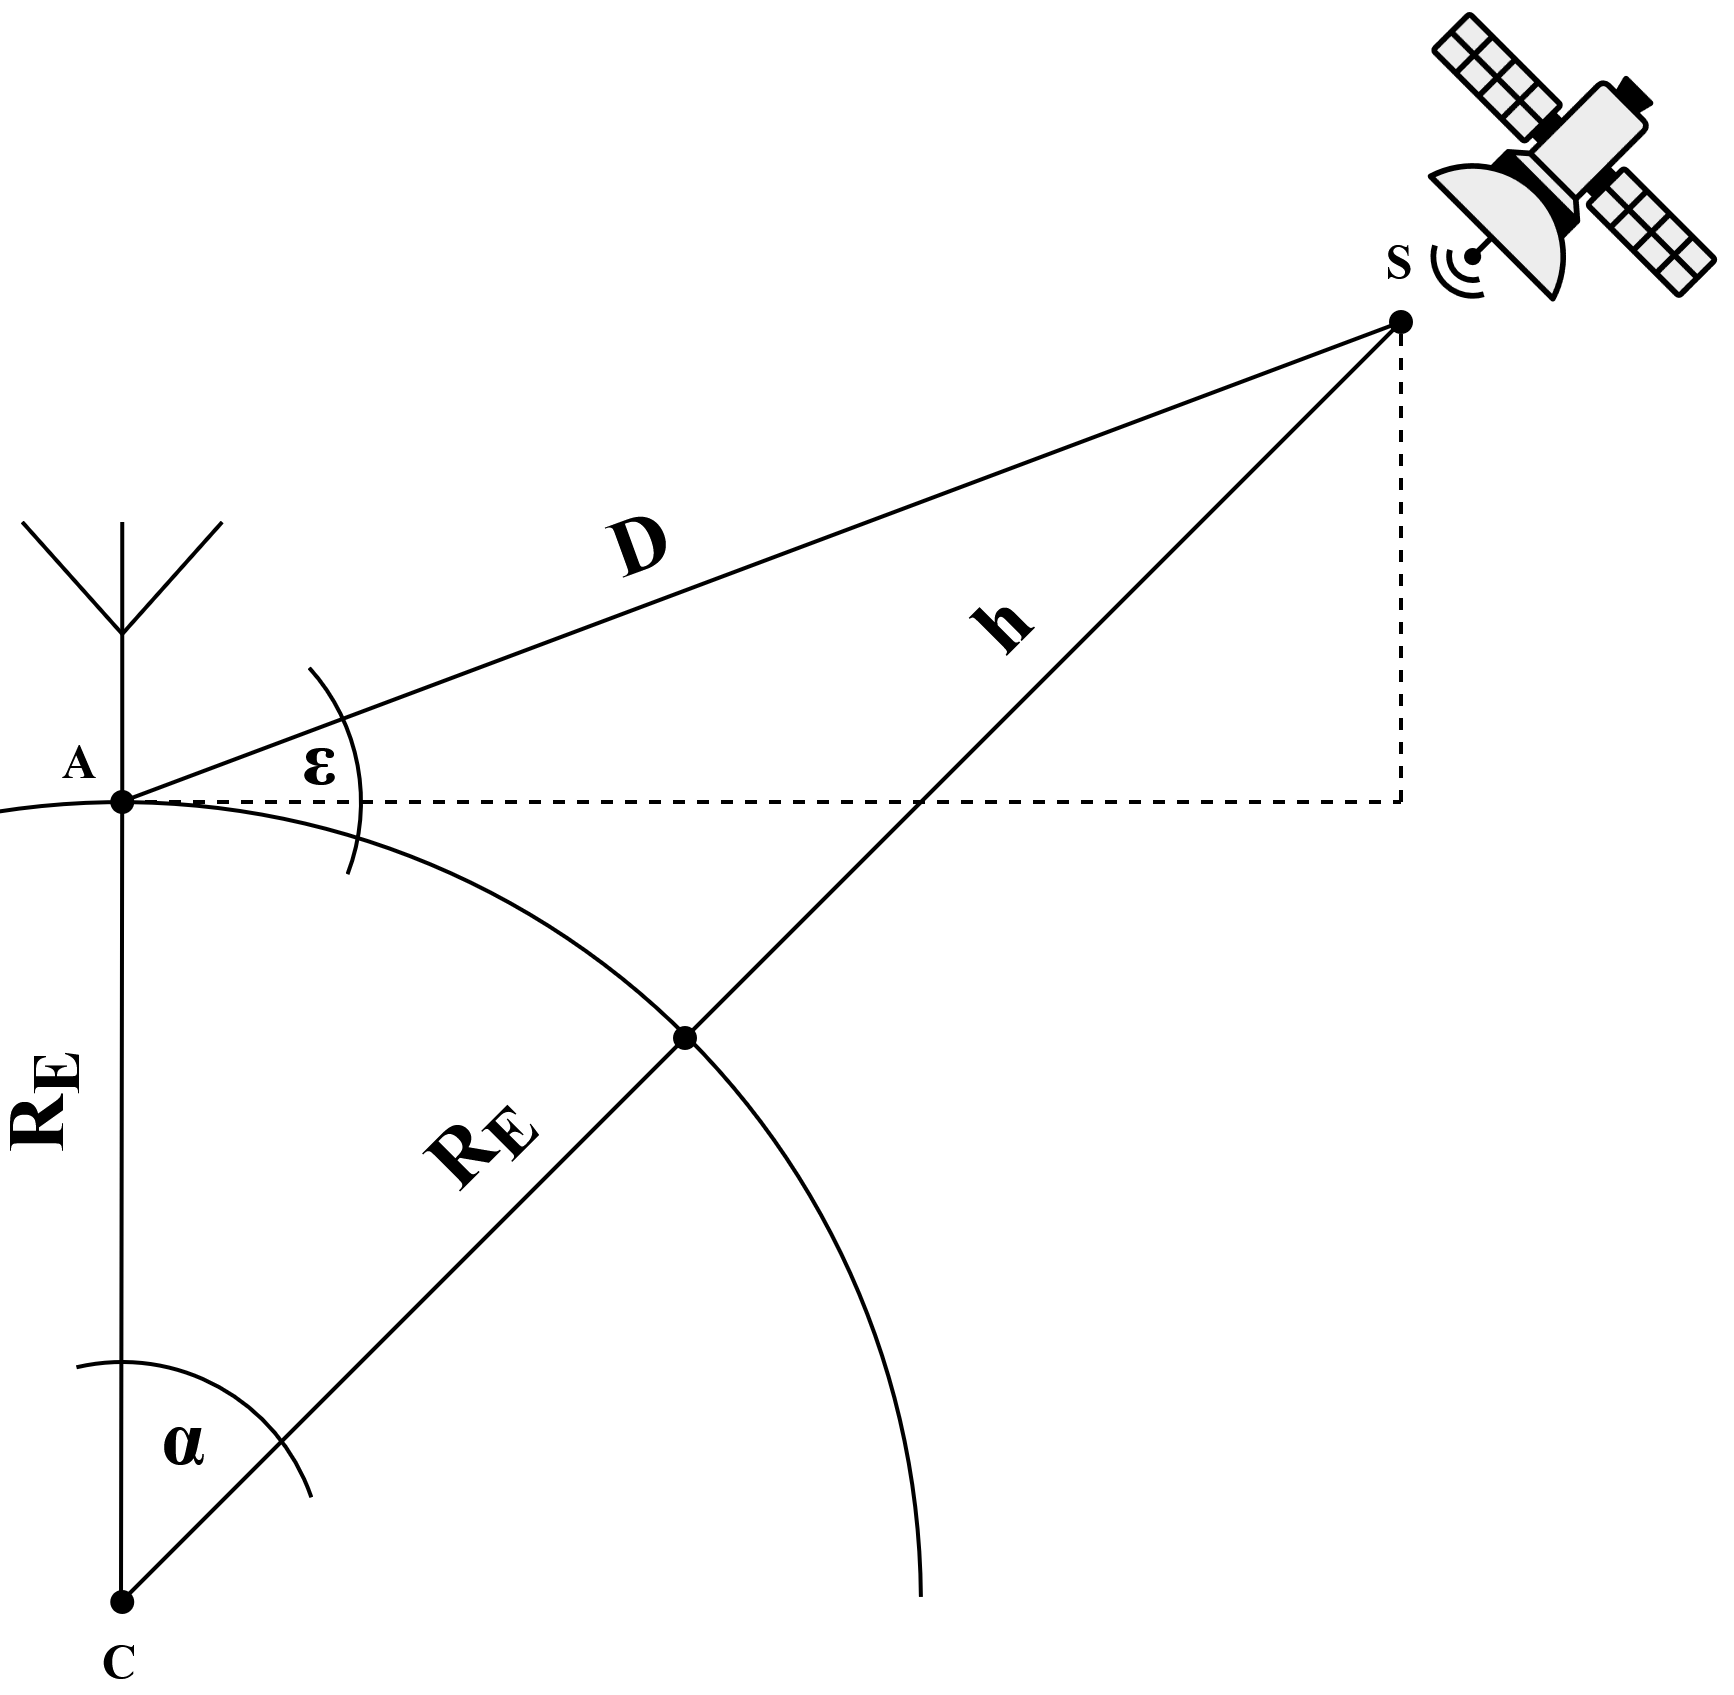
\includegraphics[width=0.7\linewidth]{Figures/slant_range.png}
    \caption{Modelo matemático para el cálculo de la distancia D en función del ángulo de elevación epsilon ($\epsilon$).}
    \label{fig:slant_range}
\end{figure}

Utilizando la ley de los cosenos sobre la geometría esférica de la Tierra, la distancia del enlace se modela rigurosamente como:

\begin{equation}
   (R_E+h)^2 = R_E^2 + D^2 - 2\,R_E\,D\,cos(\epsilon + \pi/2)
    \label{eq:ley_cos}
\end{equation}

Reemplazando $cos(\epsilon+\pi/2)$ por $-sen(\epsilon)$, luego resolviendo la ecuación cuadrática para la variable D y operando matemáticamente se obtiene la expresión:

\begin{equation}
    D(\epsilon) = \sqrt{(R_E + h)^2 - (R_E \cos\epsilon)^2} - R_E \sin\epsilon
    \label{eq:geometria_orbita}
\end{equation}

Como las pérdidas de espacio libre no contemplan efectos disipativos, se deben incluir en el balance de potencias las pérdidas debidas a la atmósfera y las deficiencias mecánicas de apuntamiento de las antenas, factores que, a diferencia de la FSPL, corresponden a pérdidas resistivas reales del trayecto y que se consolidan en la pérdida total de trayecto ($L_{path}$):

\begin{equation}
    L_{path}(\epsilon) \text{ [dB]} = L_{FSL}(\epsilon) + L_{point} + L_{atm}
    \label{eq:pérdidas_totales}
\end{equation}

Consecuentemente, el nivel de señal recibida (\textit{received signal level}, RSL) en función del ángulo de elevación, análogo a la diferencia entre el EIRP y la pérdida total de trayecto corregida por la ganancia neta de recepción, se determina mediante:

\begin{equation}
    \text{RSL}(\epsilon) \text{ [dBW]} = \text{EIRP} - L_{path}(\epsilon) + G_{rx} - L_{rx}
    \label{eq:rsl_formal}
\end{equation}

% ------------------------------------------------------------------------ %
\subsection{Modelado del Ruido y Calidad del Enlace}
La viabilidad del enlace digital no se limita a la amplitud de la portadora recibida, sino a su relación respecto a la densidad espectral de potencia de ruido térmico presente en el sistema ($N_0$), modelado como ruido blanco gaussiano aditivo. En sistemas terrestres, este ruido suele caracterizarse mediante la figura de ruido del receptor referida a una temperatura estándar de 290\,K, sin embargo, en estaciones terrenas de comunicaciones satelitales la antena recibe directamente el ruido de cielo, sustancialmente menor a 290\,K, por lo cual resulta más preciso emplear una temperatura total de sistema en lugar de una figura de ruido equivalente. Bajo este criterio, la temperatura total de ruido del sistema receptor ($T_{sys}$) se descompone aditivamente de acuerdo con el teorema de uniones en cascada, simplificado para los componentes críticos del segmento terreno:

\begin{equation}
    T_{sys} = T_{ant} + T_{LNA}
    \label{eq:tsys}
\end{equation}

donde $T_{ant}$ es la temperatura de ruido equivalente de la antena, que captura la radiación de fondo cósmico y el ruido térmico terrestre captado por los lóbulos secundarios, y $T_{LNA}$ es la temperatura de ruido efectiva referida a la entrada del amplificador de bajo ruido. La densidad espectral de ruido resultante se expresa logarítmicamente como:

\begin{equation}
    N_0 \text{ [dBW/Hz]} = k_{dB} + 10 \log_{10}(T_{sys})
    \label{eq:n0_log}
\end{equation}

donde $k_{dB} = -228{,}6 \text{ dBW/(K}\cdot\text{Hz)}$ es la expresión logarítmica de la constante de Boltzmann.

La evaluación final del desempeño del enlace digital requiere la determinación de la relación entre energía de bit disponible y densidad espectral de ruido ($E_b/N_0$), la cual se obtiene dividiendo la potencia de señal por la tasa de bits para obtener la energía por bit ($E_b = S/R_b$) y la potencia de ruido total por el ancho de banda equivalente para obtener la densidad espectral ($N_0 = N/B$), de modo que $E_b/N_0 = (S/N)(B/R_b)$. En términos del balance de enlace ya formulado, esta relación disponible en función del ángulo de elevación se expresa como:

\begin{equation}
    \frac{E_b}{N_0}(\epsilon) \text{ [dB]} = \text{RSL}(\epsilon) - N_0 - 10\log_{10}(R_b)
    \label{eq:ebn0_rb}
\end{equation}

donde el único parámetro de la cadena de transmisión digital que interviene en la ecuación es la tasa de bits $R_b$, con independencia de cómo esta haya sido determinada. En sistemas con asignación espectral rígida, $R_b$ no constituye un parámetro libre sino una cantidad derivada del ancho de banda ocupado ($BW$) y de las características del esquema de modulación. La tasa de símbolos (\textit{symbol rate}, $R_s$) en baudios se deduce a partir del factor de roll-off $\alpha$ del filtro de coseno realzado empleado para conformar el espectro, dado que la relación entre el ancho de banda ocupado y la tasa de símbolos para este tipo de filtrado responde a:

\begin{equation}
    R_s = \frac{BW}{1 + \alpha}
    \label{eq:rs_bw}
\end{equation}

A partir de la eficiencia espectral del esquema de modulación lineal M-PSK implementado, la tasa de bits efectiva queda determinada por la cantidad de bits por símbolo ($\log_{2}M$):

\begin{equation}
    R_b = R_s \log_{2}(M) = \frac{BW}{1 + \alpha} \log_{2}(M)
    \label{eq:rb_deducido}
\end{equation}

de modo que, bajo un ancho de banda constante, el aumento en el orden de la modulación $M$ incrementa la tasa de transmisión a costa de una reducción proporcional en el $E_b/N_0$ disponible por bit, según se desprende de sustituir \eqref{eq:rb_deducido} en \eqref{eq:ebn0_rb}.

El valor de $[E_b/N_0]_{req}$ que interviene en el criterio de cierre del enlace no es un parámetro arbitrario, sino que depende exclusivamente de dos factores: el esquema de modulación digital empleado y la tasa de error de bit (BER) objetivo de la misión. Esta dependencia se establece a través de la función de error complementaria gaussiana, comúnmente expresada mediante la función $Q(z)$, que es la herramienta analítica para poder vincular la relación señal a ruido disponible con la probabilidad de error de detección en presencia de ruido.

\begin{equation}
    Q(z) = \frac{2}{\sqrt{\pi}} \int_{z}^{\infty} e^{-t^2}\, dt
    \label{eq:funcion_q}
\end{equation}

Para un esquema de modulación M-PSK, sujeto a detección coherente sobre un canal AWGN, la tasa de error de bit puede aproximarse en función de $E_b/N_0$ mediante:

\begin{equation}
    \text{BER} \approx \frac{2}{\log_{2}(M)}\, Q\!\left( \sqrt{2 \log_{2}(M)} \, \sin\!\left(\frac{\pi}{M}\right) \sqrt{\frac{E_b}{N_0}} \right)
    \label{eq:ber_mpsk}
\end{equation}

expresión que, al ser invertida numéricamente para una BER objetivo preestablecida, permite obtener el valor de $[E_b/N_0]_{req}$ correspondiente a cada orden de modulación $M$. De esta manera, modulaciones de mayor orden, que ofrecen una mayor eficiencia espectral al transmitir más bits por símbolo, exigen simultáneamente una relación $E_b/N_0$ más elevada para sostener la misma tasa de error, lo cual constituye el compromiso fundamental entre velocidad de transmisión y robustez frente al ruido que se evalúa a lo largo de este balance de enlace.

Para asegurar la robustez del enlace ante desvanecimientos repentinos o imprecisiones, el margen operativo instantáneo $M_{arg}(\epsilon)$ frente al requerimiento teórico de la modulación empleada ($[E_b/N_0]_{req}$) debe superar un umbral mínimo preestablecido ($M_{min}$):

\begin{equation}
    M_{arg}(\epsilon) = \frac{E_b}{N_0}(\epsilon) - [E_b/N_0]_{req} \ge M_{min}
    \label{eq:margen}
\end{equation}

El cumplimiento de esta desigualdad define analíticamente el ángulo de elevación mínimo de visibilidad operativa $\epsilon_{min}$, por debajo del cual el enlace se considera no viable para la comunicación con la modulación correspondiente.

% ------------------------------------------------------------------------ %
\section{Implementación Computacional y Simulación}
Con el propósito de validar los rangos de operación del amplificador de potencia diseñado y determinar los límites físicos de la comunicación, se desarrollaron dos herramientas en lenguaje Python que implementan las ecuaciones~\eqref{eq:eirp_analitico} a \eqref{eq:margen}, utilizando interfaces gráficas interactivas basadas en la biblioteca \textit{Tkinter} e integración de cálculo numérico vectorizado con \textit{NumPy} y visualización mediante \textit{Matplotlib}.

El primer programa desarrollado (\texttt{link\_budget.py}) evalúa la viabilidad del enlace fijando una tasa de bits (\textit{bit rate}) analítica única y configurable para todo el sistema. El \textit{script} barre el vector de ángulos de elevación $\epsilon \in [0^\circ, 90^\circ]$ y calcula, mediante la ecuación~\eqref{eq:ebn0_rb}, una única curva de $E_b/N_0$ disponible en función de la elevación; dado que la tasa de bits es común a todo el sistema, esta misma curva se contrasta simultáneamente contra los tres umbrales requeridos ($[E_b/N_0]_{req}$ de QPSK, 8-PSK y 16-PSK), determinando para cada modulación el primer índice angular que satisface el criterio de cierre de la ecuación~\eqref{eq:margen}.

El segundo programa (\texttt{link\_budget\_bw.py}) refina el análisis adaptándolo a las limitaciones físicas de canalización del transceptor. Este algoritmo toma como variables de entrada el ancho de banda ocupado en radiofrecuencia ($BW$) y el factor de roll-off del filtro ($\alpha$), a partir de los cuales calcula una tasa de símbolos común mediante la ecuación~\eqref{eq:rs_bw} y, posteriormente, deriva una tasa de bits específica para cada esquema de modulación multiplicando dicha tasa de símbolos por la cantidad de bits por símbolo correspondiente ($2$ para QPSK, $3$ para 8-PSK y $4$ para 16-PSK), de acuerdo con la ecuación~\eqref{eq:rb_deducido}. A diferencia del primer \textit{script}, en este caso cada modulación posee su propia tasa de bits efectiva y, en consecuencia, su propia curva de $E_b/N_0$ disponible en función de la elevación, calculada de forma independiente mediante la ecuación~\eqref{eq:ebn0_bw}; el resultado son tres curvas diferenciadas, y no una curva única contrastada contra tres umbrales, lo cual modela fielmente el compromiso entre el orden de la modulación, la velocidad de transmisión resultante y la degradación del margen disponible frente al ruido térmico.

Los parámetros de simulación nominales cargados por defecto en ambas herramientas informáticas, representativos de la arquitectura física del CubeSat y el segmento terreno en banda S, se consolidan en la Tabla~\ref{tab:parametros_scripts}.

\begin{table}[H]
    \centering
    \caption{Parámetros de diseño y simulación empleados en los scripts de cálculo de radioenlace.}
    \label{tab:parametros_scripts}
    \begin{tabular}{lccc}
        \hline\hline
        \textbf{Parámetro del Sistema}             & \textbf{Símbolo} & \textbf{Valor}  & \textbf{Unidad} \\
        \hline
        Frecuencia de Operación                    & $f$              & $2{,}2$         & GHz  \\
        Radio de la Órbita Satelital               & $h_{orb}$        & $600$           & km   \\
        Ancho de Banda de Canal                    & $BW$             & $10{,}0$        & MHz  \\
        Factor de Roll-off del Filtro              & $\alpha$         & $0{,}35$        & ---  \\
        Tasa de Bits de Referencia                 & $R_b$            & $500$           & kbps \\
        Potencia de Salida del Transmisor          & $P_t$            & $0{,}0$         & dBW  \\
        Pérdidas en la Línea del Transmisor        & $L_{tx}$         & $1{,}0$         & dB   \\
        Ganancia de la Antena Transmisora          & $G_{tx}$         & $5{,}0$         & dBi  \\
        Pérdidas por Apuntamiento de Antena        & $L_{point}$      & $1{,}0$         & dB   \\
        Pérdidas por Atenuación Atmosférica        & $L_{atm}$        & $1{,}0$         & dB   \\
        Ganancia de la Antena Receptora            & $G_{rx}$         & $25{,}0$        & dBi  \\
        Pérdidas en el Sistema Receptor            & $L_{rx}$         & $1{,}0$         & dB   \\
        Temperatura de Antena                      & $T_{ant}$        & $55$            & K    \\
        Temperatura de Ruido del LNA               & $T_{LNA}$        & $120$           & K    \\
        Margen Establecido                         & $M_{min}$        & $1{,}0$         & dB   \\
        \hline\hline
    \end{tabular}
\end{table}

A continuación, las Figuras~\ref{fig:grafico_bitrate} y \ref{fig:grafico_bw} ilustran las curvas de desempeño obtenidas mediante las interfaces gráficas implementadas para cada una de las metodologías analizadas.

\begin{figure}[H]
    \centering
    \caption{Curva de $E_b/N_0$ disponible frente a elevación para una tasa de bits constante ($R_b = 500\text{ kbps}$) generada por el script \texttt{link\_budget.py}.}
    \label{fig:grafico_bitrate}
\end{figure}

\begin{figure}[H]
    \centering
    \caption{Curvas diferenciadas de $E_b/N_0$ disponible por modulación para un ancho de banda fijo ($BW = 10\text{ MHz}$) generadas por el script \texttt{link\_budget\_bw.py}.}
    \label{fig:grafico_bw}
\end{figure}